\documentclass[paper=A4,bibliography=totocnumbered]{scrartcl}
\setkomafont{disposition}{\normalcolor\bfseries} %in KOMA headings are default sans serif, with this patch with serifs see scrguide.pdf, 2010-09-14, page 108
\usepackage[dvipsnames]{xcolor}
\usepackage[latin1]{inputenc} % correct coding for windows e.g. with umlauts
\usepackage[T1]{fontenc}
\usepackage{paralist} % compactenum and compactitem
\usepackage[pdftex]{graphicx} % required to insert figures
\usepackage{listings} % format code
\lstset{escapeinside={<@}{@>}}
\usepackage[margin=10pt,font=small,labelfont=bf,labelsep=endash,singlelinecheck=false,format=plain]{caption} % formatting of captions
\usepackage{booktabs} %for professional tables using \toprule, \midrule, \bottomrule
\usepackage[round]{natbib} % http://merkel.zoneo.net/Latex/natbib.php for author-year citation with round brackets
\usepackage{vmargin} % for margins, especially bottommargin smaller, alternative to DIV=12
\setmarginsrb{35mm}{20mm}{25mm}{15mm}{12pt}{11mm}{0pt}{11mm}

% math packages
\usepackage{amsmath}
\usepackage{amssymb}
\usepackage{centernot}
\usepackage{leftidx}

% set up chapter depths
\newcommand{\subsubsubsection}[1]{\paragraph{#1}\mbox{}\\}
\setcounter{secnumdepth}{4}
\setcounter{tocdepth}{4}
\usepackage{subfig}
\usepackage[hidelinks]{hyperref} % linked pdf, necessarily at the end of preamble!!!

%##########################################################
%###################### Help! #############################
%##########################################################
% 
% Strg+T to comment a block 
% 
% \citet --> Mustermann et al. (2042)
% \citet* --> Mustermann, Musterfrau and Musterkind (2042)
% \citep --> (Mustermann et al. 2042)
% \citep* --> (Mustermann, Musterfrau and Musterkind 2042)
% 
% Insert a picture called xxx.png which is stored in the folder pic as a png
%\begin{figure}
%	\centering
%	\includegraphics[width=13cm]{pic/xxx}
%	\caption[Short Title]{Caption insert here}
%	\label{fig:somelabelname}
%\end{figure}
%
%##########################################################
%########### End Preferences, Begin Document ##############
%##########################################################

%opening
\title{Programming Project 03}
\author{Francel Lamprecht, Christine Robinson, Regina Wehler}
\date{Winter Semester 2018/19}

\begin{document}

\maketitle

\tableofcontents
\clearpage
\section{Introduction}
Plant phenotyping is a research  area in the plant sciences that focuses on the quantitative measurement of both functional and structural properties of plants. During the last decade plant phenotyping evolved to non-destructive, image-analysis-based phenotyping. This computer driven approach allows the characterization of plants in a high-throughput manner \citep{Walter.2015}.

The focus of this plant phenotyping research project was on the processing, segmentation and classification of \textit{A.~thaliana}, to gain valuable insight on how the image-analysis-based phenotyping in the life sciences works. \textit{A.~thaliana} is often used as a model plant, as the plant is small in size, with a rapid life cycle of about six weeks \citep{Koornneef.2010}. 

The project was divided into two main parts:
a) Image Analysis with Fiji in Java
b) Explorative Data Analysis with Python in Jupyter Notebook.

\section{Methodology}
The images used in this project are from the Leaf Segmentation Challenge. These images were supplied to the challenge by the International Plant Phenotyping Network (IPPN).
Each image was processed in a consecutive series of algorithms and tools which are implemented as plugins in the Fiji distribution \citep{Schindelin.2012} of the open-source software ImageJ \citep{Rueden.2017}. The image analysis approach consists of three main steps (figure \ref{fig:pipeline}). First, the input RGB input image is segmented into two classes, plant and background by a trainable Weka segmentation classifier. Second, the binary class output is used to identify single leaf objects by watershed segmentation. The resulting binary mask is utilized to analyze properties of the leaf objects in the single red, green and blue channel, respectively.

\begin{figure}
	\centering
	\subfloat[Input]{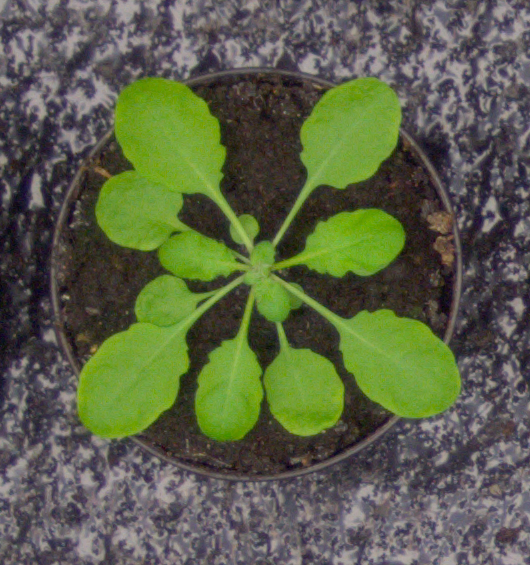
\includegraphics[width=.3\textwidth]{pic/27_rgb}}
	\qquad
	\subfloat[Classification]{
\includegraphics[width=.3\textwidth]{pic/27_class}}
	\qquad
	\subfloat[Watershed]{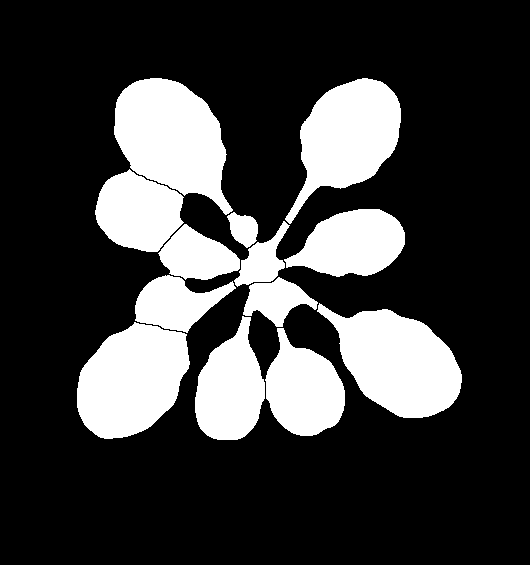
\includegraphics[width=.3\textwidth]{pic/27_watershed}}
	\qquad
	\subfloat[Particle Analysis]{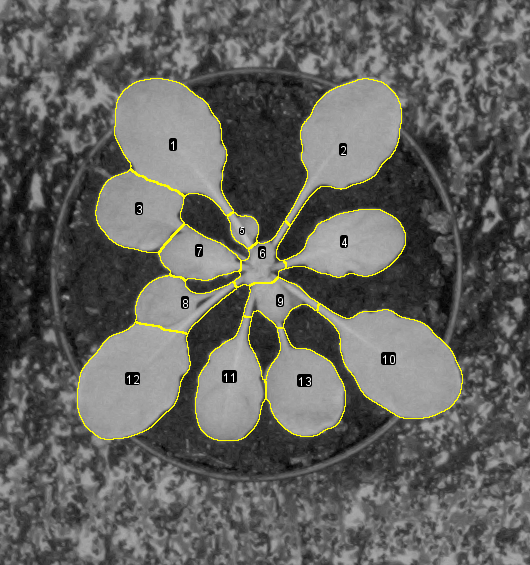
\includegraphics[width=.3\textwidth]{pic/27_greenPA}}
	\caption[Image analysis pipeline]{The analysis of plant leaves is conducted in three steps. The RGB input image (a) is classified into plant and background by a trainable Weka segmentation classifier (b). Single leaf objects are identified by watershed segmentation (c). The binary mask is used to analyze properties in the split red, green and blue channel (d).}
	\label{fig:pipeline}
\end{figure}

\subsection{Segmentation}
The plant is separated from the background with the help of a trainable Weka segmentation classifier \citep{ArgandaCarreras.2017}. Weka provides a GUI to train machine learning algorithms to produce pixel-based segmentations. The user can add traces to classes and train the classifier with those. Afterwards, traces/regions of interest can be adjusted and the classifier can be re-trained to improve classification. Six representative pictures are selected from the 2017 data set for training (plant029, plant145 and plant159 from A1; plant032, plant034 and plant037 from A2). Pictures are chosen to cover the whole range of plant green shades and the range of background characteristics of the given data sets. The Weka Experimenter was used to assess the performance of different machine learning algorithms. Based on these results (table \ref{tab:weka}), FastRandomForest was used with default parameters as a classifier. By applying the trained classifier to the RGB input images, for each input image a binary classification image is obtained (figure \ref{fig:pipeline}-b). 

\begin{table}[htbp]
	\centering
	\caption{Comparison of classifier performance by Weka Experimenter. The default algorithm parameters were kept.}
	\begin{tabular}{lllllll}
		\toprule
		Algorithm & Percent correct & Precision & Recall & F score & Matthews  & AUC \\
		 & & & & & correlation & \\
		 \midrule
		FastRandomForest & 99.93 & 1.00 & 1.00 & 1.00 & 1.00 & 1.00 \\
		SMO & 92.52 & 0.89 & 0.93 & 0.91 & 0.85 & 0.93 \\
		$k$-nearest Neighbors & 95.38 & 0.95 & 0.93 & 0.94 & 0.90 & 0.95 \\
		RandomSubSpace & 99.85 & 1.00 & 1.00 & 1.00 & 1.00 & 1.00 \\
		Bagging & 99.77 & 1.00 & 1.00 & 1.00 & 1.00 & 1.00 \\
		DesicisonTable & 99.05 & 0.99 & 0.9 & 0.99 & 0.98 & 1.00 \\
		\bottomrule
	\end{tabular}
	\label{tab:weka}
\end{table}

\subsection{Objects Recognition}
A plant consists of leaves that are attached to each other. To be able to analyze leaves individually, they need to be separated. Here, the watershed algorithm was used to separate touching objects. Its implementation in Fiji is based on the algorithm described by \citet{Kunt.1990}. The algorithm first calculates an Euclidean distance map and determines center points as points which are, from a topological view, the ultimate eroded points, As the algorithm's name indicates, this topological map is "flooded" with water and at each collision of two "watersheds", a line separating two objects is drawn. Before watershed was applied, outliers were removed in both classes of the binary image by using the Fiji remove outliers function separately on each class. This function uses a median filter, for which the pixel radius was set to 6 and the threshold was set to 50. The output of the watershed algorithm is the binary image with added watershed lines (figure \ref{fig:pipeline}-c). 

\subsection{Object Analysis}
After an image was subjected to the aforementioned steps, the resulting watershed image was then analyzed using Fiji's Analyze Particles tool. The measurements that were selected to be performed during the particle analysis are:

\begin{compactitem}
\item Area - Measures the area of selection in square pixels. This was used to obtain the object's size.
\item Mean gray value - Average gray value of the selection.
\item Centroid - Provides the center point of the selection as the average X and Y coordinates for all pixels in the selection or image.
\item Bounding rectangle - This is the smallest possible rectangle that encloses the selection. It gives the X and Y coordinates in respect of the upper left corner of the rectangle, as well as the height and width, from which the width-to-height-ratio will be calculated.
\item Shape descriptors - These descriptors are used to attain the roundness of each object.
\item Feret's diameter - Can be used to find the longest distance between any two points on the selection boundary.
\item Integrated density- Used to indicate the sum of the brightness, as it sums the values of the pixels in the image or selection
\end{compactitem}

Particles with a pixel size less than 70 were excluded from the "Analyze Particles" command. The value of 70 was established by trial and error, by inspecting the lines drawn by the watershed algorithm to separate objects.

Fiji automatically generates a Results Table, with the selected measurements. These results can be accessed by using the \texttt{getResultsTable()} method in the source code, to select the appropriate results for further use. By using this method, a csv file with all the results deemed necessary was created. 

The generated Results Table results ("columns") that were included in the csv file can be seen in Table \ref{tab:result_table}.

\begin{table}[htbp]
	\centering
	\caption{Measurement options and the corresponding value in the csv file.}
	\begin{tabular}{lll}
		\toprule
		Measurement option  & Corresponding value in the csv file \\
		\midrule
		 Display Labels & objectID and imageID\\
		Area & size\\
		Centroid & pos\_x and pos\_y\\
		Shape descriptors & roundness\\
        Integrated density & brightness\_sum\\
      	Mean gray value & brightness\_average\\
       	Bounding rectangle & width\_to\_height\_ratio\\
        \bottomrule
	\end{tabular}
	\label{tab:result_table}
\end{table}

As brightness values calculated from binary watershed images is insufficient for plants, Fiji's "Analyze Particles" command was also applied to the original RGB images. The brightness (both the sum and the average) of each of the three color channels (red, green and blue) were individually calculated. These individual channel results were then added together to calculate the sum of the brightness and average brightness for each object. To ensure computational efficiency not all the measurements were selected again, as this would have resulted in the duplication of results, eg. the size of the objects will remain constant, it is independent of the type of input image. The measurements that were necessary to be applied to the original RGB images, are the mean gray value and the integrated density. Results regarding the brightness of each color channel were attained and added to the csv file. 

An additional requirement of the project was to include the width to height ratio. As this is not a built-in measurement option in Fiji, the width and the height that were included in the Results Table, as part of the "Bounding rectangle" measurement were extracted and the ratio was calculated, by dividing the leaf width by the leaf height. The calculated width to height ratio was added to the csv file to be available for further use. 

\subsection{Explorative Data Analysis}
Data analysis was conducted in Jupyter Notebooks using several Python packages. Data were handled with the python package pandas. For visual statistical analysis, the seaborn package was used. Numerical statistical analysis was mainly performed using the stats module from the python package scipy. For general plotting of graphs, the pyplot module from the python package matplotlib was used.

\subsection{Data}
For this study, datasets of the Leaf Segmentation and Counting Challenges were used \citep{Minervini.2016}. The imaging data were manually annotated to provide ground truth information \citep{Scharr.2014}. The datasets contain images of greenhouse images with \textit{A.~thaliana} and \textit{N.~tabacum}. \textit{A.~thaliana} is a rosette plant, with the individual leaves being on separate, distinguishable stems. This characteristic of \textit{A.~thaliana} makes leaf separation from each other less complex.  Given that we were only exploring viable methods in this research area, \textit{A.~thaliana} was our chosen plant, as it gave us the opportunity to explore with different algorithms in an easier way than what the \textit{N.~tabacum} dataset would have allowed us to do. Since the datasets for 2014, 2015 and 2017 are nearly the same, only differing in the amount of provided meta data, datasets from a single year were used for analysis. 

\section{Results}
\subsection{Overview of the 2014 datasets}

\begin{figure}
	\centering
	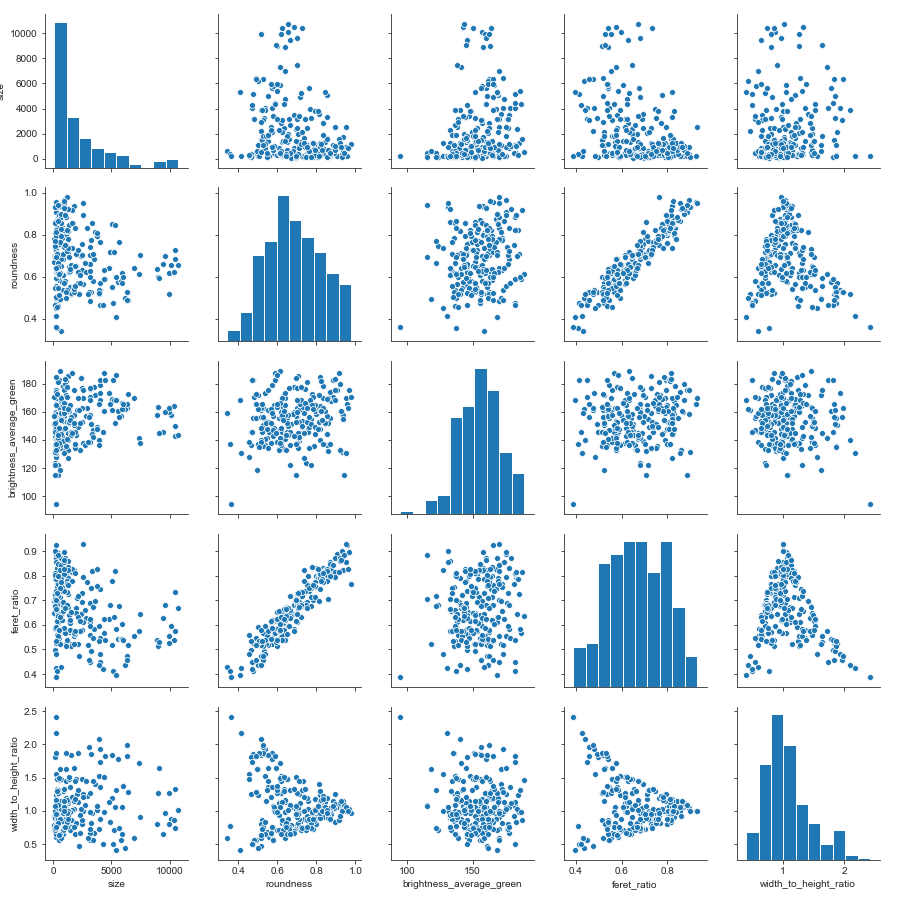
\includegraphics[width=13cm]{pic/overview}
	\caption{Overview of correlations in the 2014 datasets shown in a pairplot matrix.}
	\label{fig:overview}
\end{figure}

\subsection{Analyses of correlations}
\begin{figure}
	\centering
	\subfloat[Size vs. Roundness]{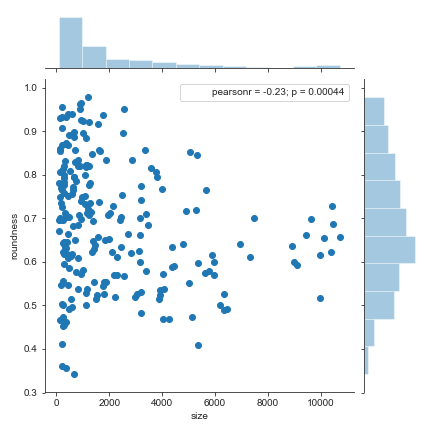
\includegraphics[width=.45\textwidth]{pic/size-roundness}}
	\qquad
	\subfloat[Size vs. Color]{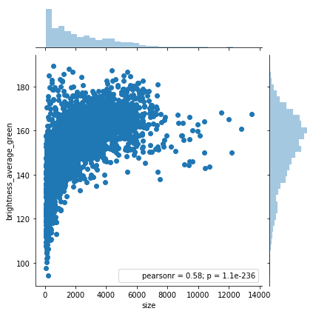
\includegraphics[width=.45\textwidth]{pic/size-color}}
	\qquad
	\subfloat[Number of Leaves vs. Total Area]{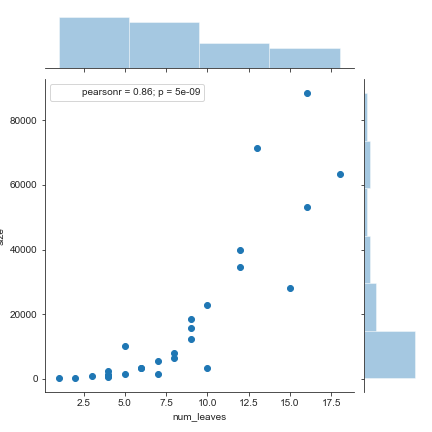
\includegraphics[width=.45\textwidth]{pic/number-area}}
	\caption{XXX}
	\label{fig:corr}
\end{figure}

- Correlation of leaf size and roundness
- Correlation of leaf size and color
- Correlation of leaf number and total plant area


\subsection{Comparison of A1 and A2 datasets}

\begin{figure}
	\centering
	\subfloat[A1 Dataset]{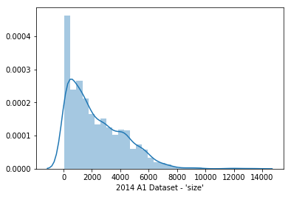
\includegraphics[width=.45\textwidth]{pic/A1-size}}
	\qquad
	\subfloat[A2 Dataset]{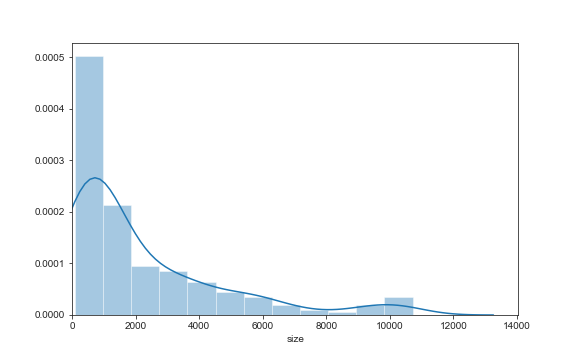
\includegraphics[width=.45\textwidth]{pic/A2-size}}
	\caption{XXX}
	\label{fig:A1-A2-size}
\end{figure}

\subsection{Comparison of leaf count to ground truth}

\begin{figure}
	\subfloat[A1 Dataset]{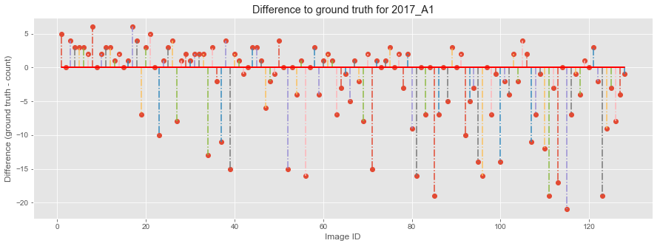
\includegraphics[scale=.5]{pic/A1-truth}}
	\qquad
	\subfloat[A2 Dataset]{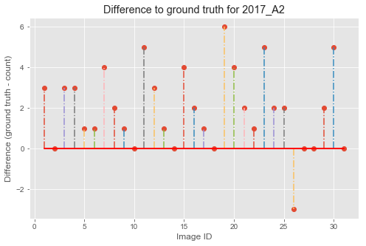
\includegraphics[scale=.5]{pic/A2-truth}}
	\caption{XXX}
	\label{fig:truth}
\end{figure}

\section{Discussion}

%TODO
%TODO Francel: Maybe we should also include sub-headings in the discussion? I know it is not standard in a "normal" thesis, but maybe for this project's it might be a good idea. I don't mind either way... :) 
%TODO Regina: sub-headings in the discussion chapter is standard. but it shouldn't be the same headings from another chapter (normally it's tempting to use the same heading from the results in the discussion). And I think that the explanation of our choice of measurements should go to the methodology chapter.**

\subsection{Challenges in the Identification of Single Leaves}
- quality of classification depends on the selection of images for training and on the selection of traces

- need to find a balance between number of labeled pixels and classification accuracy because with increasing number of labeled pixels the reading of the classifier later requires more time

- watershed is working best for circular objects, that's why it sometimes fails on leaves with long stems

- detection and removal of outliers is difficult for very small plants -> with our pipeline we have lost very small plants (pixel number?)

\subsection{Object Analysis}
%TODO ** REMOVE THIS COMMENT. Discussion of where we needed to decide which measurement to include in results table/csv file. Not discussing the obvious ones. I think that is clear in the methodology section. Only discussing the position (also asked in assignment) and roundness vs circularity**

Most of the decisions made about which measurements to include in the Fiji generated Results Table became clear when reading the ImageJ documentation. \citep{Ferreira.2012}. One decision that was needed to be made, was whether to take an object's position from the the top left appearing pixel or from the centroid. In this project we used the centroid to indicate the object's position, as by using the top left appearing pixel position has no advantage over the centroid. By using the centroid positions, we ensured that the position coordinates are more robust to possible rotations. If the top left appearing pixel was used, problems could arrive if the leaves were to be rotated. 

In  the Fiji Results Table, circularity and roundness are two similar measurements. Circularity in ImageJ is calculated in such a way that it excludes local irregularities 
%TODO \citep{Wirth.2004} If I'm not taken wrong, these are powerpoint slides. I don't think we are allowed to use those as a source... 
, therefore the roundness measurement which gives a value directly relative to the aspect ratio, was included in the csv file.



\renewcommand\bibname{References} % necessarily before \bibliography{ref}, but not working in preamble
\bibliographystyle{apalike} % for references chapter
\bibliography{ref}

\end{document}
